%&pdflatex
\documentclass[10pt,border=5pt]{standalone}
\usepackage[utf8]{inputenc}
\usepackage[T2A]{fontenc}

\usepackage{tikz}

\usetikzlibrary{arrows,decorations.pathreplacing}

\begin{document}

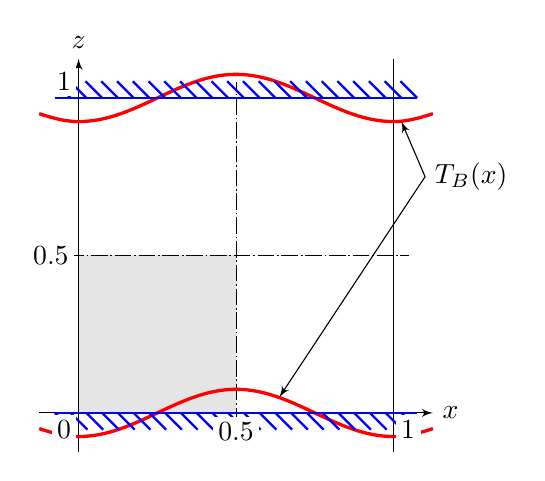
\begin{tikzpicture}[dashdot/.style={dash pattern=on .6pt off 1pt on 6pt off 1pt},
            interface/.style={postaction={draw, decorate, decoration=
                {border, angle=-45, amplitude=0.3cm, segment length=2mm}}},
            label/.style={fill=white, inner sep=2pt},
            >=latex', scale=1]
    \fill[gray!20] (0,0) -- (2,0) -- (2,2) -- (0,2) -- cycle;
    \draw[->] (-.5,0) -- (4.5,0) node[right] {\(x\)};
    \draw[->](0,-.5) -- (0,4.5) node[above] {\(z\)};
    \draw(4,-.5) -- (4,4.5);
    \draw[dashdot] (-.2,2) -- (4.2,2);
    \draw[dashdot] (2,-.2) -- (2,4.2);
    \draw[red, very thick] (-.5,-.2) sin (0,-.3) cos (1,0) sin (2,.3) cos (3,0) sin (4,-.3) cos (4.5,-.2);
    \draw[red, very thick] (-.5,3.8) sin  (0,3.7) cos (1,4) sin (2,4.3) cos (3,4) sin (4,3.7) cos (4.5,3.8);
    \draw[blue, thick, interface](-.3,0) -- (4.3,0);
    \draw[blue, thick, interface](4.3,4) -- (-0.3,4);
    \draw[<->] (4.1,3.7) -- (4.4,3) node[right] {\(T_B(x)\)} -- (2.55,.2);
    \node at (-.02,-.02) [below left, label] {0};
    \node at (4.02,-.02) [below right, label] {\(1\)};
    \node at (-.02,4.02) [above left, label] {\(1\)};
    \node at (-.05,2) [left, label] {\(0.5\)};
    \node at (2,-.05) [below, label] {\(0.5\)};
\end{tikzpicture}

\end{document}
